This chapter introduces the concepts necessary to understanding the subject of this thesis.
We aim to:
\begin{itemize}
    \item present the central pieces of an \emph{agent-based approach} in artificial intelligence: agent and environment;
    \item explain how we can reason about problems using this paradigm;
    \item introduce key concepts in the field of \emph{reinforcement learning (RL)};
    \item describe \emph{Q-learning} and how we can use neural networks to improve the classic algorithm;
    \item exemplify a successful application of this approach.
\end{itemize}

\section{AI and Intelligent Agents} \label{agents-intro}
The concept of rational agent is central to the study of artificial intelligence. 
It is a natural evolution to the \textit{laws of thought} approach in AI (using a set of logical rules to derive new knowledge).

As pointed out in \cite{aima}, inference does not capture all of rationality.
As complex environments imply \textit{uncertain situations} (where there is no provably correct choice to make), a finite set of rules can prove inadequate.
The agent-based approach captures a more complete definition of rationality by shifting focus from making correct inferrences to producing \emph{efficient behaviour}.

\subsection{Definition. Agent Function and Agent Program}
According to \cite{aima}, an \textbf{agent} is simply something that percieves and acts in an environment.
An agent can be split into two major components, each fulfilling a fundamental function:
\emph{perceptors} (sensors) manage \emph{perception} and \emph{actuators} act upon the environment.
This is the simplest useful division. We present a more elaborate division later, in Section \ref{learning-agents}.

It is sometimes useful to reason about agents in a mathematical space.
For this, there exists the concept of \emph{agent function}.
An \textbf{agent function} maps what the agent percieves (every ``snapshot'' of perception, called a \emph{percept}) to an action.
Outside the world of very small, ideal examples, any agent function can be considered \emph{infinite}.
The implementation of an agent function is an \textbf{agent program}, which is what AI is actually concerned with building and perfecting.
This implementation is, of course, finite.

The term \emph{agent} \textbf{can} designate physical robots working in real-life environments.
However, in this paper we use the term \textit{agent} to refer exclusively to softbots (or software robots).
The problem that we solve can be entirely modeled in a virtual space.

\subsection{Task Environments}
Simply put, \textbf{task environments} are a way to express a problem to which an agent is the solution.
The design of the agent depends on the attributes of its environment.

In this paradigm, we can decompose a task into several subcomponents, often abbreviated \textbf{PEAS}\cite{aima}, comprising of:
\begin{enumerate}
    \item \textbf{performance measure}, a function which measures the performance of the agent;
    \item \textbf{environment}, the ``world'' the agents interacts with;
    \item \textbf{actuators}, the agent's means of action;
    \item \textbf{sensors}, the agent's means of perception;
\end{enumerate}

The \textbf{performance measure} has many possible representations, depending on the problem.
Its primary purpose is to measure how effective the behaviour of the agent is, with regard to the given goals.
In reinforcement learning, we measure this effectiveness using a \textbf{reward function}.
We will elaborate on this in our section on reinforcement learning (Section \ref{reinforcement-learning}).

\subsubsection{Environment Classification}

Modeling real-world use cases requires understanding the vast diversity of environments.
In the following paragraphs, we present some \textbf{classification criteria} for task environments that are also provided in \cite{aima}.

\textbf{Observability} can be \emph{full} or \emph{partial}.
In a fully observable environment, the agent has full information of all the relevant aspects of the world (for example, a chess-playing agent sees the entire chessboard).
The latter means the agent operates with restricted information.
Many real-world problems have partial observability due to sensor noise or memory/CPU constraints.

\textbf{Single- or multi-agent}.
Multi-agent environments are a tool for studying emergent behaviour, wherein relatively simple agents construct elegant and complex solutions to problems.
The techiques concerning the design of multi-agent systems are frequently subtle and can be treated as another subject completely.

\textbf{Stochasticity}.
In a \emph{deterministic} environment, every state is completely determined by its previous. Otherwise, the environment is \emph{stochastic}. An environment is \textbf{uncertain} when it is stochastic and/or partially observable.

\textbf{Discreteness} and \textbf{continuity}.
This is best understood by example:
in a game of chess, a chess-playing agent has a finite number of possible actions.
Chess is therefore a discrete environment.
An agent driving a car, on the other hand, has control over some real-valued parameters of the car (steering angle, speed and so on).
Thus, the domain of possible actions in real-world driving is continuous.
In this example, we used discreteness and continuity to describe the domain of available actions.
The same property describes \emph{time} inside the environment: in discrete time, time spent deciding does not influence the outcome. The opposite is true for continuous time representation. Coming back to our driving analogy -- every second spent not making a decision is stalling.

\textbf{Known} and \textbf{unknown}.
This refers to the agent's knowledge of the laws governing its environment. In a known environment, the agent knows the rules of its world a priori. Otherwise, an agent has to learn how the environment works in order to make effective decisions.

% Can include environment classes and environment generators

\subsection{Learning Agents} \label{learning-agents}
In this paper, we are intereseted in creating an autonomous learning agent.
An agent system would be useless by modern standards if it had no capacity to \textbf{learn from past experience}.
In this section, we aim to understand learning agents by going through the anatomy of their system.
It is worth mentioning that the actual architecture of the program will not be a one-to-one match to this conceptual tour.

Russel and Norvig provide an excellent description of \textbf{learning} in intelligent agents in \cite{aima}:
\begin{quote}
    Learning in intelligent agents can be summarized as a process of modification of each component of the agent to bring the components into closer agreement with the available feedback information, thereby improving the overall performance of the agent.
\end{quote}

In our chapter introduction (Section \ref{agents-intro}) we said that agents have an advantage over knowledge-based approaches.
This advantage comes from the fact that agents can learn in initially \textbf{unknown environments}.
Learning allows agents expand on initial knowledge, if any.
Learning agent approaches can achieve substantial results starting with \textbf{zero expert knowledge}, as shown by AlphaZero\cite{alpha-zero}.

According to \cite{aima}, an agent can be divided in four subsystems:
\begin{enumerate}
    \item \textbf{the learning element}, which is resposible for improving the agent;
    \item \textbf{the performance element}, which selects actions (this part is the object of improvement);
    \item \textbf{the critic}, which provides feedback to the learning element;
    \item \textbf{the problem generator}, which suggests novel actions, in order to expand knowledge.    
\end{enumerate}

A learning agent overview figure, closely following the schematic provided in \cite{aima}, is shown in Figure \ref{fig:aima-learning-agent}.

\begin{figure}[ht]
    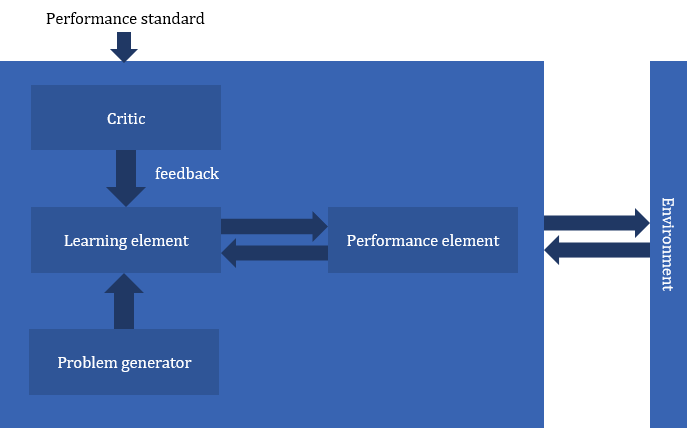
\includegraphics{aima_learning_agent}
    \centering
    \caption{An overview schematic of the learning agent system.}
    \label{fig:aima-learning-agent}
\end{figure}

\subsubsection{Learning and Performance}
The performance elements provides the basic function of the agent: it perceives, decides and acts.
The learning element's job is to improve this performance based on feedback, coming from an outside observer (the critic).
The learning element's design varies depending on the problem and how the agent is meant to interact with it.
One common example of implementation is a \emph{neural network}.
We will see how deep learning comes into play in Chapter \ref{deep-q-learning}.

\subsubsection{The Critic}
An agent cannot tell whether its behaviour is effective just by observing changes in the environment.
It needs a \textbf{critic} that provides feedback to the learning element about its performance in the world.
The critic can esentially be viewed as a stand-alone, external entity.
It is based on a fixed performance standard which does not depend on the agent's internal state.
In fact, it is imperative for the critic to be kept separate of agent state.
This prevents the agent of ``deluding'' itself that it is doing a good job.

\subsubsection{The Problem Generator}
Agents can get stuck making decisions that yield good but suboptimal results (local optima, a well-known problem in AI).
This happens because the agent bases its calculations on limited knowledge.
It needs a component to take care of adding new information into its system.
The problem generator solves this problem of \textbf{exploration}:
choosing options that yield suboptimal results in the short term, in order to discover better strategies on the long term.


% Link to brainstorming https://docs.google.com/document/d/1Dk2yzwWefNas-AZOo0nMAd4xbwd7LNU9qV0miYcRuBc/edit

% But what are those components? Dive in: learning element, performance element, critic, problem generator
% Add a figure

% 1/4 OF CHAPTER 1 COMPLETE

\section{Reinforcement Learning} \label{reinforcement-learning}
% Here we introduce many fundamental notions of reinforcement learning
% Include a case study of AlphaGo

\section{Q-Learning}
% Here we start by describing naive Q-learning

% then we introduce deep Q-learning
% in this subsec, we will also do a quick introduction to neural networks

\section{Deep Q-Learning} \label{deep-q-learning}

% Here we do a rundown of possible improvements of Q-learning: Double Q-learning and Duelling Q-learning

% Include a case study of DQN in the original Atari paper